\documentclass[convert={outfile=\jobname.png}]{standalone}
\usepackage{base}

\begin{document}

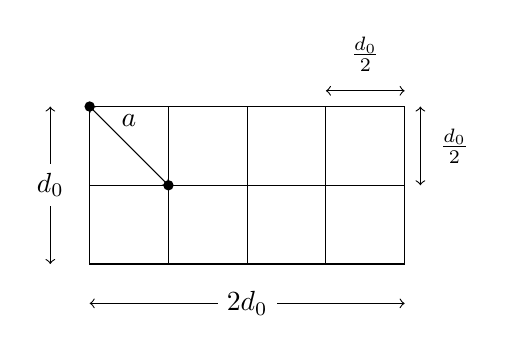
\begin{tikzpicture}
    \draw(0, 0) rectangle (4,2);
    \draw(0, 1) -- (4, 1);
    \foreach \x in {1, 2, 3}
       \draw(\x, 0) rectangle (\x, 2);
    \draw[<->] (0, -.5) to node[fill=white] {$2d_0$} (4, -.5);
    \draw[<->] (-.5, 0) to node[fill=white] {$d_0$} (-.5, 2);
    \draw[<->] (3, 2.2) to node[label=above:$\textstyle\frac{d_0}{2}$] {} (4, 2.2);
    \draw[<->] (4.2, 1) to node[label=right:$\textstyle\frac{d_0}{2}$] {} (4.2, 2);
    \draw[<->] (0, 2) node[fill=black, circle, scale=.4] {} to node[label=$\textstyle{a}$] {} (1, 1) node[fill=black, circle, scale=.4] {};
\end{tikzpicture}

\end{document}
